\section{Ziel}
Das Ziel dieses Versuchs ist es, verschiedene Eigenschaften eines $LRC$-Schwingkreises
anhand von erzwungenen bzw. gedämpften Schwingungen zu untersuchen.

\section{Theorie}
\label{sec:Theorie}
\cite{V354}

\subsection{Amplitude einer gedämpften Schwingung}
% Amplitude einer gedämpften Schwingung mit Dämpfungswiderstand 
Die Spannung lässt sich im Allgemeinen als Differentialgleichung darstellen.
Nach dem 2. Kirchhoffschen Gesetz gilt für die Spannung in einer Masche,
also einem Schaltkreis, dass die Summe aller Spannungen gleich Null ergeben muss:
\begin{align*}
    U_{R}(t)+U_{C}(t)+U_{L}(t) &= 0 
\end{align*}
Dabei ist $U_{R}(t)$ die zeitlich veränderliche Spannung an dem Widerstand $R$,
$U_{C}(t)$ die Spannung am Kondensator mit Kapazität $C$ und $U_{L}(t)$ die Spannung
an der Spule mit Induktivität $L$, also die induktive Spannung.
Für die gedämpfte Schwingung ergibt sich die Gleichung:
\begin{equation}
    I(t)= A_{0} e^{-2 \pi \mu t} \cos(2 \pi \nu t + \eta),
\end{equation}
wobei $2 \pi \mu = \frac{R}{2L}$ ist. $I$ ist die Stromstärke, $A_{0}$ der Startwert,
$\nu$ die Frequenz und $\eta$ eine Phasenverschiebung.
Die Abklingdauer ist durch
\begin{equation}
    T_{ex} = \frac{1}{2 \pi \mu} = \frac{2L}{R}
    \label{eqn:t_ex}
\end{equation}
gegeben.
Der effektive Dämpfungswiderstand bestimmt sich durch
\begin{equation}
    R_{eff} = 4 \pi \mu L.
    \label{eqn:reff}
\end{equation}

\subsection{Aperiodischer Grenzfall}
%R(aperiodischer Grenzfall) Formel mit Amplitude, Schwingungsdauer und was sonst aus a gegeben ist 
Beim aperiodischen Grenzfall geht die Spannung ohne Überschwingung am schnellsten gegen null
(gestrichelte Linie Abb. \ref{fig:ap_gr}). Dieser kann durch die Gleichung
\begin{equation} 
    I(t)=A e^{-\frac{R}{2L}*t}= A e^{-\frac{t}{\sqrt{LC}}}
\end{equation}
beschrieben werden.
Der Dämpfungswiderstand dabei ist gegeben durch
\begin{equation}
    R_{ap} = \sqrt{\frac{4L}{C}}.
    \label{eqn:r_ap}
\end{equation}
\begin{figure}
  \centering
  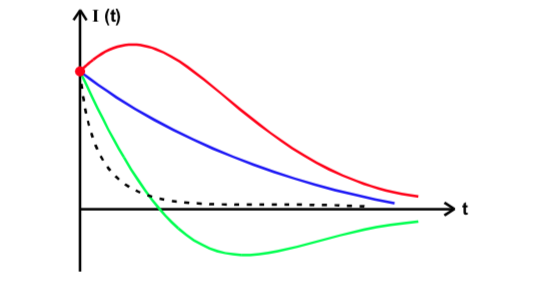
\includegraphics[width= 10cm, height= 7cm]{build/ap_grenzfall.png}
  \caption{Mögliche zeitliche Verläufe des Stroms in einem Schwingkreis mit aperiodischer Dämpfung.}
  \label{fig:ap_gr}
\end{figure}

\subsection{Frequenzabhängigkeit der Kondensatorspannung}
%Frequenz zu Kondensatorspannung Verbindung
Die Abhängigkeit der Kondensatorspannung von der Kreisfrequenz
\begin{equation*}
    \omega = 2\pi f
\end{equation*}
der Erregerspannung lässt sich mittels 
\begin{equation}
    U_{C}(\omega)= \frac{U_{0}}{\sqrt{(1-LC\omega^{2})^{2} + (\omega R C)^{2}}}
\end{equation}
beschreiben.
Bei dem Phänomen der Resonanz erreicht $U_{C}$ ein Maximum, das über der Amplitude $U_{0}$ der Erregerspannung liegt:
% Frequenz zu Erreger und Kondensatorspannung, bzw. die jeweiligen Spannung in ihrer Verbindung zu einander
\begin{equation}
    U_{C, max} = \frac{1}{\omega_{0}RC} U_{0} = q U_{0} = \frac{1}{R} \sqrt{\frac{L}{C}} U_{0}.
    \label{eqn:ucmax}
\end{equation}
$U_{C}$ überschreitet bzw. unterschreitet die Erregerspannung also um den Faktor 
\begin{equation}
    q = \frac{1}{\omega_{0}RC} = \frac{1}{R} \sqrt{\frac{L}{C}}.
    \label{eqn:q}
\end{equation}
Dieser Faktor ist die Güte, bzw. Resonanzüberhöhung.
Daraus lässt sich die Breite der Resonanzkurve bestimmen:
\begin{equation}
    \frac{U_{C}(\omega_+)}{U_0} = \frac{U_{C}(\omega_-)}{U_0} = \frac{q}{\sqrt{2}}.
    \label{eqn:breite}
\end{equation}
% \begin{equation}
    % \omega_{+} - \omega_{-} = \frac{\omega_{0}}{q}.
    % \label{eqn:breite}
% \end{equation}

\subsection{Frequenzabhängigkeit der Phase}
Die Phase in Abhängigkeit von der Frequenz der Erregerspannung wird durch
\begin{equation*}
    \varphi(\omega) = \arctan(-\frac{\omega RC}{1-LC\omega^2})
\end{equation*}
beschrieben.
Sie lässt sich auch anhand des Abstands der Nulldurchgänge $\delta t$ zweier Schwingungen beschreiben:
\begin{equation}
    \varphi = \frac{\delta t}{T} 2 \pi.
    \label{eqn:phi}
\end{equation}
Dabei ist $T$ die Schwingungsdauer, die sich mittels
\begin{equation*}
    T = \frac{1}{f}
\end{equation*}
aus der Frequenz ergibt.
Die Resonanzfrequenz ist gegeben durch
\begin{equation}
    \omega_{res} = \sqrt{\frac{1}{LC} - \frac{R^2}{2L^2}}.
    \label{eqn:omega_res}
\end{equation}
An den Stellen $\frac{\pi}{4}$ oder $\frac{3}{4} \pi$ gilt für die Frequenzen $\omega_{1}$
und $\omega_{2}$:
\begin{equation}
    \omega_{1,2} = \pm \frac{R}{2L} + \sqrt{\frac{R^2}{4L^2} + \frac{1}{LC}}.
    \label{eqn:omega_12}
\end{equation}
Die Differenz bzw. die Breite der Resonanzkurve ist also
\begin{equation}
    \omega_+ - \omega_- = \frac{R}{L}.
    \label{eqn:diff}
\end{equation}